%================================================================
%                           N O T E S
%                           ---------
%
%                           ---------
%================================================================
%                       INTRODUCTION
%================================================================
%   TODO: insert diagram of problem
%   TODO: write better introduction to the problem once it's done - sort of like the abstract but specific to this chapter (include applying boundary conditions etc)
%   TODO: why must they all satisfy the helmholtz equation?
%   TODO: redo hand drawn diagrams
%   TODO: am I defining the wave vector correctly?
%   TODO: why is phi a function of ax+by?
%   TODO: is the harmonic condition the same as the helmholtz equation?
%   TODO: move to small case phi since it's 2D and not 3D
%   TODO: separation of variables to solve 2.1
%----------------------------------------------------------------
\section{Introduction to the problem}
For this problem we consider a plane wave propagates from infinity onto a cylinder centered at the origin and of radius $\sigma$, as depicted in \figref{fig:problem_1}. We will attempt to find an expression for the velocity field of this wave as it scatters around the cylinder. We will consider two different boundary conditions, Neumann and Dirichlet, and will find expressions for both of these. \par
%
    \begin{figure}
        \centering
        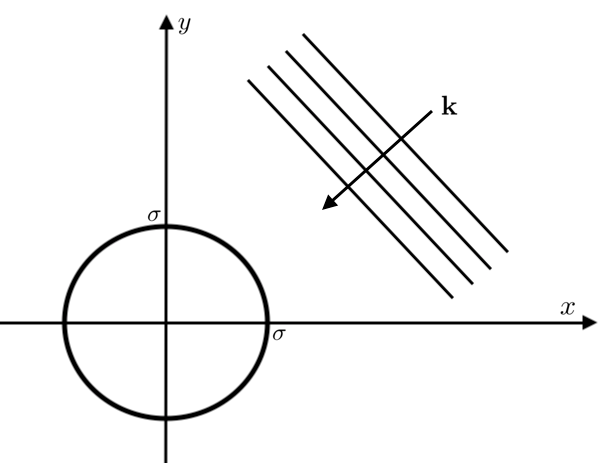
\includegraphics[width=6cm]{prob1/prob1_figures/sk_problem_1.png}
        \caption{Problem 1}
        \label{fig:problem_1}
    \end{figure}
%
We will use the following definitions throughout this problem. \par
%
    \begin{defn}
    The \emph{wave vector} $\vec{k}$ of a 2D plane wave is defined as
        \[ \vec{k} = (a, b) = (k\cos\alpha, k\sin\alpha)
        \]
    where $k$ is the \emph{wave number} and $\alpha$ is the \emph{incident angle} of the wave as shown in \figref{fig:incident_wave}. Note that $k^2=a^2+b^2$.
    \end{defn} \par
%
Physically, the wave number corresponds to the number of oscillations per unit distance, and is inversely proportional to the wavelength $\lambda$.\par
%
In \ssref{ss:separation_of_vars} we defined $\omega=kc$, where $c$ is the speed of sound. This has a physical interpretation.
    \begin{defn}
    The frequency of a plane wave with wave vector $\vec{k}$ is $kc= \omega$.
    \end{defn}
    \begin{equation}
        k = \frac{2\pi}{\lambda} = 2\pi
    \end{equation}
%----------------------------------------------------------------
%               deriving incident wave function
%----------------------------------------------------------------
    \section{Inncident wave function}
The incident wave is a plane wave with wave vector $\vec{k}$, and incident angle $\alpha$. The magnitude of the wavevector is the wave's wavenumber, $k$. Hence $\vec{k} = (k \sin\alpha, k \cos\alpha)$.
    \begin{figure}  %------- incident wave sketch ---------------
        \centering
        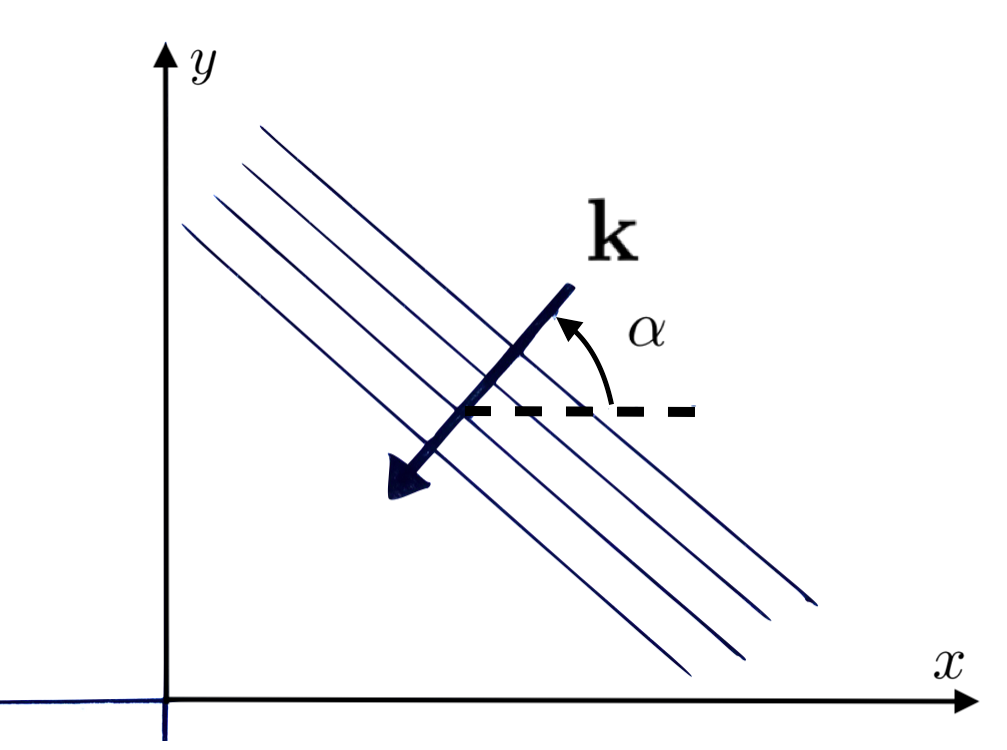
\includegraphics[width=6cm]{prob1/prob1_figures/sk_incident_wave_2.png}
        \caption{Incident wave with wavevector $\vec{k}$}
        \label{fig:incident_wave}
    \end{figure}

    \begin{defn}    %-------------- definition ------------------
    The wavenumber $k$ of an acoustic wave is the number of oscillations per unit distance. It is inversely proportional to its wavelength $\lambda$:
    \[
    k = \frac{2 \pi}{ \lambda} = 2 \pi \frac{c}{\omega}.
    \]
    Where $c$ is the speed of sound. 
    \end{defn}
Note that this definition shows that $k \in \bb{R}.$

We can see that this field is made up of straight lines. We therefore pose that $\phi(x,y) = \phi(ax + by)$ for $a$ and $b$ real constants. From \ref{eq:harmonicity_condition} we know that $\phi$ must satisfy:
    \begin{equation*}
        \nabla^2 \phi + k^2 \phi = 0
    \end{equation*}
    \begin{equation}
        \partialfrac{^2 \phi}{x^2} + \partialfrac{^2 \phi}{y^2} + k^2 \phi = 0
    \end{equation}
We can break up this partial differential equation into two ordinary differential equations:
%this is separation of variables
    \begin{multicols}{2}
    \noindent
    \begin{equation}
        \frac{d^2 \phi_x (x)}{dx^2} + k^2 \phi_x (x) = 0
    \end{equation}
    \begin{equation}
        \frac{d^2 \phi_y (y)}{dy^2} + k^2 \phi_y (y) = 0
    \end{equation}
    \end{multicols}
Since we know that $k \in \bb{R}$, particular solutions are $e^{-iax}$ and $e^{-ibx}$ respectively, for $a,b \in \bb{R}$. Hence a particular solution for $\phi(x,y)$ is $e^{-i(ax + by)}$. Figure \ref{fig:plane_wave} shows the plots of the real and imaginary parts of $\phi$ for $a,b = 1$. 
    \begin{figure}[ht]  %----------- plots ----------------------
        \centering
        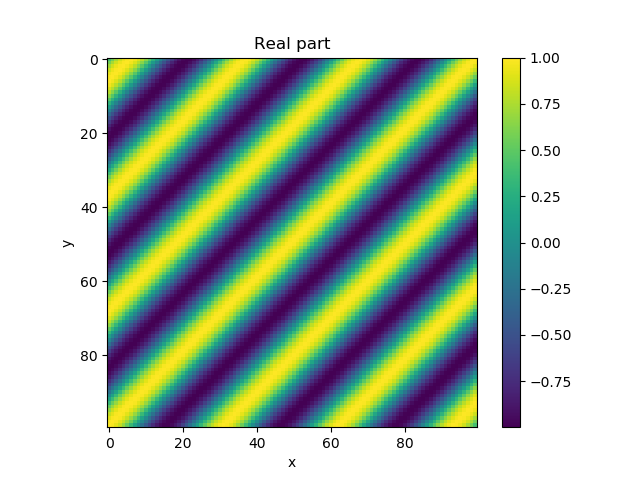
\includegraphics[width=6cm]{prob1/prob1_figures/py_plane_wave_real_part.png}
        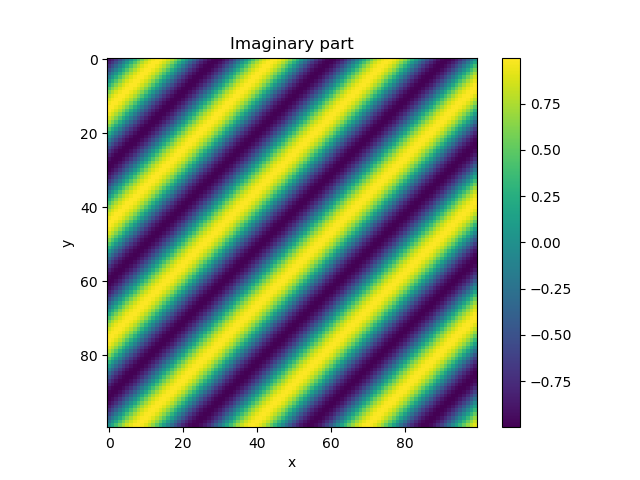
\includegraphics[width=6cm]{prob1/prob1_figures/py_plane_wave_imaginary_part.png}
        \caption{Countour plot for the real and imaginary parts of $e^{-i(x+y)}$, see \ref{lst:plane_wave}.}
        \label{fig:plane_wave}
    \end{figure}

%================================================================
%                       SCATTERED FIELD
%================================================================
%   TODO: why is it valid that phitot is a linear combination of phiin and phiscattered
%   TODO: diagram showing shadow area etc
%   TODO: why is separation of variables valid here? Maybe check under what conditions separation of variables is valid
%   TODO: bessel function for kr, not just r
%   TODO: can I call theta dependence azimuthal dependence?
%   TODO: go into more detail on solutions of bessel equation
%   TODO: how to reference bessel and hankel functions properly since its all taken from the same book
%   TODO: go through derivation of solution zwillinger chapter 108
%   TODO: change notation, f(r) -> R(r), g(theta) -> Theta(theta)
%   TODO: get to hankel solution from bessel and neumann combined solution 
%   TODO: prove that most general solution of f(r) is linear combination.
%   TODO: why are A, B functions of n and R?
%----------------------------------------------------------------
    \section{Deriving the scattered field}
We can describe the total field $\Phitot$ in terms of the incident field, $\Phiin$, and the scattered field, $\Phisc$.
    \begin{equation}
        \Phitot = \Phiin + \Phisc
    \end{equation}
All three of these, $\Phitot, \Phiin, \Phisc$, must satisfy the Helmholtz equation. 

%----------------------------------------------------------------
%               separation of variables
%----------------------------------------------------------------
\subsection{Separation of variables}\label{ss:separation_of_vars}
We want to find an expression for $\Phisc$. For this we use separation of variables.
    \begin{equation}\label{phi_scattered_separation}
        \Phisc (r, \theta) = f(r)g(\theta)     
    \end{equation}
We know that \ref{phi_scattered_separation} must satisfy \ref{eq:harmonicity_condition}, that is
    \begin{equation}
        \nabla^2 \Phisc + k^2 \Phisc = 0.
    \end{equation}
Hence,
    
The expression inside the brackets depends only on $r$ and $g''/g$ depends only on $\theta$, therefore they both must equal the same constant $\nu^2$. \\

%----------------------------------------------------------------
%                   theta dependence, g(theta)
%----------------------------------------------------------------
\subsection{Solving for \texorpdfstring{$\theta$}{theta} dependence}

\begin{equation}\label{phi_scattered_eigenvalue}
    g''(\theta) - \nu^2 g(\theta) = 0
\end{equation}

This is an eigenvalue problem. There are three possible cases for $\nu$: $\nu^2=0$, $\nu^2 < 0$ or $\nu^2 > 0$. Note that we expect our solution to be $2\pi$ periodic, since it depends on $\theta$, the polar angular coordinate.\\

\textbf{Case 1:} $\nu = 0$. This gives a solution of the form $c \theta + b$, which is not $2 \pi$ periodic. \\
\textbf{Case 2:} $\nu^2 > 0$. This gives a solution of the form $A e ^{\nu \theta} + B e^{- \nu \theta}$, which is also not $2 \pi$ periodic. \\
\textbf{Case 3:} $\nu^2 < 0$, where a particular solution is $g_0(\theta) = A_0 \cos (\nu \theta) + B_0\sin( \nu \theta)$. 
%TODO: explaint this next step in detail

Therefore we get a general solution:
\begin{equation}
    g(\theta) = \sum_{n=0} ^\infty A_n \cos (n \nu \theta) + B_n \sin (n \nu \theta) 
\end{equation}
Where $A_n = A_n(n, R) $ and $B_n = B_n (n, R)$, where $R$ is the radius of the cylinder.
%TODO: check whether this eqtn is right 

%----------------------------------------------------------------
%               bessel and hankel functions
%----------------------------------------------------------------


%----------------------------------------------------------------
%               r dependence
%----------------------------------------------------------------
\subsection{Solving for \texorpdfstring{$r$}{r} dependence}
We will use these Bessel functions to find a general solution for the $r$ dependence of our scattered field. In \ref{ss:separation_of_vars}, we arrived at the following differential equation.
    \begin{gather*}
       r^2 \frac{f''}{f} + r \frac{f'}{f} - k^2r^2 = n^2
    \end{gather*}
    \begin{equation}
        r^2 f'' + r f' -(k^2r^2 + n^2)f = 0
    \end{equation}
Which has solution
    \begin{equation}
        f(r) = A J_{n}(kr) + B Y_{n}(kr)
    \end{equation}
for $J_n$ and $Y_n$ Bessel and Neumann functions respectively \cite[Chapter~108]{zwillinger92handbook}.

%================================================================
%                   BOUNDARY CONDITIONS
%================================================================
%   TODO: two types: dirichlet and neumann. Go into detail
%----------------------------------------------------------------
%\section{Boundary conditions}
%----------------------------------------------------------------
%                   radiation condition
%----------------------------------------------------------------
%\subsection{Radiation condition}
%----------------------------------------------------------------
%                       dirichlet bc
%----------------------------------------------------------------
%\subsection{Dirichlet boundary conditions}
%----------------------------------------------------------------
%                       neumann bc
%----------------------------------------------------------------
%\subsection{Neumann boundary conditions}

%================================================================
%                       PLOTTING
%================================================================
%   TODO: all
%----------------------------------------------------------------
%\section{Plotting}